\documentclass[a4paper,12pt]{article}
%\usepackage[spanish]{babel} % espanol
\usepackage[utf8]{inputenc} % acentos sin codigo
\usepackage{graphicx} % graficos 
\usepackage[none]{hyphenat} % evitar separación de palabras entre lineas
\usepackage{lscape} % para insertar páginas en horizontal
\usepackage{rotating}
\usepackage{multirow}
\usepackage{cite}
\usepackage{flushend}
%\usepackage{anysize} % para ajustar márgenes de página
%\usepackage{afterpage}
\hyphenation{po-ly-a-cry-la-mi-de} % configura cómo debe partirse siempre esta palabra
\author{Miguel Ángel Martín Piedra}
\title{Cell viability and proliferation capability of long-term human dental pulp stem cell cultures for use in tissue engineering.}
\date{2017}
\addcontentsline{toc}{section}{References}
\begin{document}
\sloppy % justificación de párrafos
\begin{titlepage}

\begin{center}
\vspace*{-1in}
\begin{figure}[htb]
\begin{center}

\includegraphics[width=10cm]{logo}
\end{center}
\end{figure}

DARWIN EVENTUR\\
\vspace*{0.6in}
\begin{large}
CURSO:\\
\end{large}
\vspace*{0.2in}
\begin{Large}
\textbf{\LaTeX y Git aplicado a la investigación científica.} \\
\end{Large}
\vspace*{0.3in}
\begin{large}
Trabajo realizado por Miguel Ángel Martín Piedra\\
\end{large}
\vspace*{0.3in}
\rule{80mm}{0.1mm}\\
\vspace*{0.1in}
\begin{large}
Profesores: \\
Renato L. Ramirez Rivero \\
Pablo Hinojosa \\
\end{large}
\end{center}

\end{titlepage}


% Página en blanco
\newpage
$\ $
\thispagestyle{empty} % para que no se numere esta pagina



%\twocolumn[ % Se aplica twocolumn en el texto, el preámbulo sólo tiene en cuenta que vas a usar el paquete, pero no lo aplica.
%\begin{@twocolumnfalse}
\tableofcontents

\maketitle % título, autor y fecha

\rule{120mm}{0.1mm}\\

\begin{abstract}
\textbf{Background:} Evaluation of cell viability is one of the most important steps of the quality control process of cells used therapeutically. The aim of this study was to evaluate the long-term cell viability profile of human dental pulp stem cells (hDPSC) subcultures (beyond 10 passages) to determine which of these passages are suitable for clinical use, and to identify the cell death processes that may occur in the last passages. \textbf{Methods:} Four different cell viability assays were combined to determine the average cell viability levels (ACVL) at each cell passage: Trypan blue exclusion test, WST-1, LIVE/DEAD and electron probe X-ray microanalysis (EPXMA). Apoptosis was assessed by TUNEL assay and caspase 4 and BCL7C western blotting, and cell proliferation was analyzed by WST-1 and PCNA protein detection. \textbf{Results:} hDPSC showed high ACVL from passages P11 to P14, with adequate cytoplasmic and mitochondrial functionality at these subcultures. A non-significant trend to decreased cell proliferation was found from P16 to P20. EPXMA and TUNEL analyses suggest that a preapoptotic process could be activated from P15 to P20 (p$<$0.001), with a correlation with caspase 4 and BCL7C expression. \textbf{Conclusions:} hDPSC corresponding to passages P11 to P14 show adequate cell function, proliferation and viability. Therefore, these cells could be considered as potentially useful for clinical applications.\\
\textbf{Keywords:} Cell viability, Dental pulp, Mesenchymal stem cells, Electron-probe X-ray microanalysis.
\end{abstract}
%\end{@twocolumnfalse}
%]

% @twocolumnfalse sirve para anular el formato de doble columna, para poner el título y el abstract, y luego se cierra @twocolumnfalse, para volver al modo twocolumn (lo que se hace es negar una afirmacion)

%\marginsize{2.5cm}{2.5cm}{2cm}{4cm}
\twocolumn
\section{Introduction}
Human dental pulp stem cells (hDPSC) have only become known from 2,000 on, and these cells have been deeply studied and characterized since then. hDPSC are considered to be the most feasible and promising stem cells derived from human teeth due to their biological properties, easy obtaining and for being present almost during the whole lifespan in the dental pulp of permanent human teeth. hDPSC are clonogenic and highly proliferative, even more than bone marrow mesenchymal stem cells. Furthermore, hDPSC are very similar to other adult mesenchymal stem cells regarding the positive expression of mesenchymal undifferentiation markers and the negative expression of CD45 \cite{RN1229}. hDPSC have high differentiation potential, showing great capabilities to differentiate to chondrogenic, osteogenic, adipogenic, but also neurogenic and even epithelial lineages. Because of this, these cells are globally considered as mesenchymal stem cells (MSC). As other stem cells, hDPSC are increasingly used in regenerative medicine, especially for the development of biological substitutes (artificial tissues) by Tissue Engineering (TE) \cite{RN1058}.\\
In this regard, it is necessary to ensure the proliferative and regenerative potential of cells used in regenerative medicine and TE protocols in order to guarantee the success of these protocols. Therefore, evaluation of cell viability is one of the most important goals of the quality control process of cells used for the generation of artificial tissues. Moreover, understanding the specific cell death mechanisms that may occur during sequential cell culturing would contribute to a better selection of the most appropriate cell sources \cite{RN287}.\\
Several methods have been used to the date to evaluate cell viability, ranging from commonly used methods based on the analysis of the integrity of the cell membrane using vital exclusion dyes such as trypan blue, to other assays focused on the study of cell metabolism such as AM calcein staining or WST-1 methods. One of the most interesting methods designed to evaluate cell viability is electron probe X-ray microanalysis (EPXMA), which allows the accurate determination of cell viability and the identification of the mechanisms underlying cell death by quantification of the ionic elements that play a key role in cell viability \cite{RN231}. This method has been extensively used for the study of cell viability of different cell types, including hDPSC. \cite{RN244}\\
\begin{center}
\begin{figure}
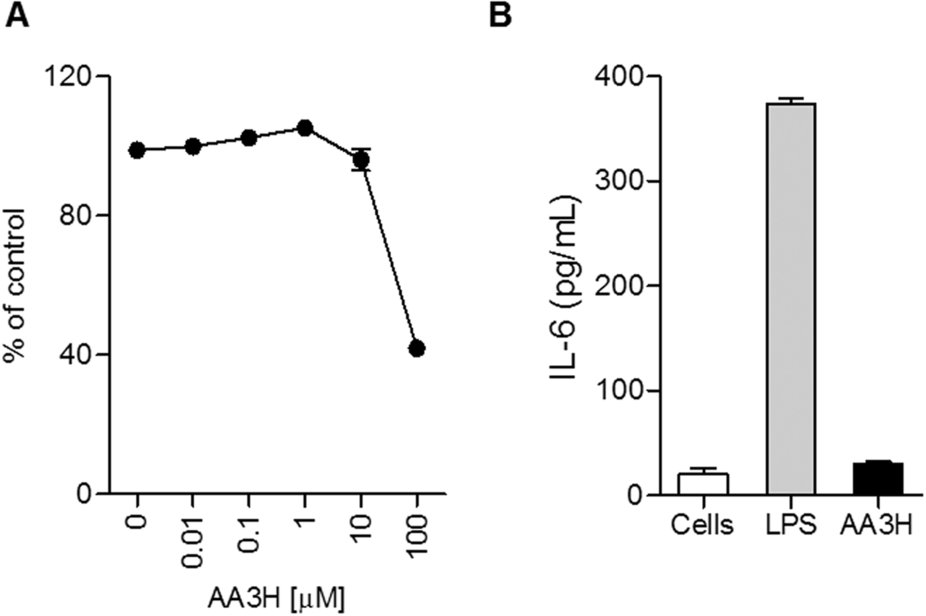
\includegraphics[width=6cm]{fig1}
\caption{Results of ERK1A5 transfection with human lentivirus protocols on dermal rat fibroblasts.}
\label{Figure 1}
\end{figure}
\end{center}

Adult stem cells cultured in laboratory for several passages tend to show a typical 3-steps cell viability profile as previously reported: (i) an initial adaptation to ex vivo cell culture conditions associated to a slight decrease of cell viability; (ii) an increasing  period, when cell viability rises and cells reach the top cell viability levels. Cells at this moment are recommended for use in regenerative medicine; and (iii) a decreasing phase, when cells tend to lose viability and cell death is present. \cite{RN628} It is not recommended to use cells at this period.\\
hDPSC viability was recently studied during the first 10 cell subcultures by using an array of cell viability assays \cite{RN923}. However, hDPSC reached the top cell viability at the end of the study (passage 9). Thus, it is necessary to go further on this type of research and to analyze long-term hDPSC subcultures (beyond 10 passages) to determine if these passages are also suitable for clinical use, and because it is important to identify those subcultures in which cells undergo active cell death and the mechanisms underlying this process \cite{RN985}. Once the cell viability profile has been evaluated, researchers will be able to choose hDPSC subcultures with optimal cell viability and proliferation, as well as to discard low-viability subcultures for therapeutic use.\\
The aim of this study was to evaluate the cell viability profile of long-term hDPSC subcultures (from 11th to 20th passages) to determine the putative usefulness of these cells and to identify the stage when hDPSC tend to lose cell viability. In addition, the mechanisms involved in cell death and its early indicators will be analyzed.
\section{Materials and Methods}
\subsection{Samples and hDPSC Cultures}
Four human dental pulps were obtained from young adult teeth (from 18 to 30 years). All these teeth were third molars without dental or periodontal pathology extracted by dental prescription at the School of Dentistry of the University of Granada. All teeth presented a fully developed root stage (closed apex stage).\\
Once extracted, teeth were stored at 4ºC in Dulbecco’s modified Eagle’s medium (Sigma-Aldrich Company, Steimheim, Germany) supplemented with 600 U/mL penicillin, 0.6 mg/mL streptomycin and 1.5 $\mu$g/mL anfotericin B (Sigma-Aldrich) and immediately processed at the Tissue Engineering Laboratory at the School of Medicine of the University of Granada.\\

Dental pulps were extracted and digested as previously described \cite{RN206}. The medium used for hDPSC culture was Dulbecco’s modified Eagle’s medium (Sigma-Aldrich) supplemented with 10\% fetal bovine serum (Sigma-Aldrich; Cat: F9665; Lot: 062M3398, St Louis, MO, USA) and 1\ antibiotic/antimycotic solution (Sigma-Aldrich). Medium was changed every 3 days and cells were subcultured at subconfluence using a 0.5 g/L trypsin and 0.2 g/L ethylendediaminetetraacetic (EDTA) solution (Sigma-Aldrich) at 37ºC for 4 min. Cells were kept in culture until the 20th passage and analyzed from passage 11 (P11) to passage 20 (P20).\\
\subsection{Trypan Blue vital dye exclusion assay.}
To determine the number of cells and their viability using trypan blue, 20 $\mu$L of trypsinized and resuspended cells were mixed with 20 $\mu$L of 0.4\% solution of trypan blue dye (Sigma-Aldrich) for 1 minute. Cells were immediately counted using a Neubauer microchamber (Brand GmbH, Wertheim, Germany) with a light microscope. All counts were done using 4 technical duplicates of each sample. Means and standard deviations were calculated for each subculture \cite{RN211}.\\
\subsection{WST-1 metabolic proliferation and cell viability assay.}
To determine the mitochondrial metabolic activity and cell proliferation of hDPSC, the WST-1 method was used as previously described \cite{RN770}. Briefly, 10,000 cells were cultured in 96-well plates (Iwaki, Japan). After subsequent subculture for 48 hours, cells were rinsed with phosphate buffered saline (PBS) and 10\% WST-1 reagent solution (Roche Diagnostics, Indianapolis, IN, USA) was added for 4 hours at 37º C. Then, each sample was analyzed using a UVM 340 plate reader (Asys, Cambridge, UK). As negative controls, selected cultured wells were previously treated with 2\% Triton X-100 (Probus, Barcelona, Spain). All counts were done using 4 technical duplicates of each sample.\\
\subsection{LIVE/DEAD® cell viability assay.}
Simultaneous evaluation of cytoplasmic function and membrane integrity was carried out by LIVE/DEAD® Viability/cytotoxicity kit for mammalian cells (Invitrogen, Oregon, USA) assay. This assay provides information about the functional status of cell by detecting the cytoplasmic sterase activity. The kit consist on two fluorescent dyes: AM calcein, which pass across the cell membrane. Once hydrolyzed by cytoplasmic sterase (live cells), calcein show fluorescence in 515 nm emission wavelength. On the other hand, ethidium homodymer only show fluorescence (617 nm emission wavelength) after binding to DNA. Thus, red fluorescence only appears in cells whose cell membrane is disrupted (dead cells). LIVE/DEAD® cell viability assay was performed using chamber slides (LabTek II, Nunc, Rochester, NY, USA). Briefly, 20,000 cells were seeded on each well and cultured for 48 h. Then, cells were rinsed twice with PBS, and cell viability was assessed using LIVE/DEAD® kit according to the manufacturer’s protocol as previously described \cite{RN46}. Cell counts were done using 6 technical duplicates of each sample.\\
\subsection{Electron probe X-ray microanalysis (EPXMA).}
For X-ray microanalysis, confluent hDPSC were subcultured using trypsin-EDTA on plated gold grids covered with a thin layer of Pioloform (polyvinyl butyral) (Ted Pella, Inc., Redding, CA) and sterilized overnight under UV light. Cells were seeded at a density of 5,000 cells per grid and cultured in DMEM supplemented with 10\% serum and antibiotics. Then, grids containing the cells were washed with deionized water at 4ºC, plunge-frozen, freeze-dried, carbon-coated and analyzed using a scanning electron microscope with a EDAX microanalytical as previously described. For each cell, the intracellular ionic concentration of Na, Mg, P, S, Cl, K and Ca, as well as the K/Na ratio were determined. 50 cells were analyzed per cell passage.
\subsection{Average Cell Viability Levels (ACVL).}
In order to calculate average cell viability levels (ACVLs) for each cell passage \cite{RN206}, the raw cell viability values as determined by trypan blue, WST-1, LIVE/DEAD® and K/Na index were first normalized to z-scores (mean=0 and standard deviation=1) using the formula: 

$$Z=\frac{X-\mu}{\sigma}$$
 
where $\mu$ is the average cell viability obtained for each method, X is the specific cell viability for a particular cell passage, and $\sigma$ is the standard deviation for each method. Then, mean z-scores values were obtained for each of the ten cell passages analyzed.

\subsection{Transferase dUTP Nick End Labeling (TUNEL) assay.}
Apoptosis of hDPSC was detected by using In Situ Cell Death Detection Kit (Roche Diagnostics, Mannheim, Germany) and following the manufacturer's instructions at passages P11, P13, P15, P17 and P19. This fluorescence assay was carried out using Chambers slides (LabTek II, Nunc, Rochester, NY, USA). Briefly, 20,000 cells were seeded on each well and cultured for 48 h. Then, cells were washed and incubated with the TUNEL enzyme and label solution. Finally, the fluorescent reaction was counterstained with DAPI and analyzed in a fluorescent microscope.\\
\subsection{Western blot and inmunofluorescence.}
To obtain whole cell protein extracts, hDPSC were collected in cell lysis buffer (Mammalian cell lysis kit, Sigma-Aldrich Ltd, Steinheim, Germany). All samples were incubated on ice for 15 min and centrifuged at 10,000 rpm for 5 min. Each protein extract was quantified using a Commassie Blue protein assay (Bio-Rad Laboratories, Hercules, CA, USA). Equal amounts of protein were loaded onto a 7.5\% polyacrylamide gel (Mini-PROTEAN© TGX, Bio-Rad Laboratories, Hercules, CA, USA) and separated by electrophoresis. Proteins were then transferred to a nitrocellulose membrane using 2.5A current for 3 min. The membrane was blocked in blocking buffer (WesternDot©, Invitrogen, Eugene, OR, USA) for 1 hour at room temperature and incubated with anti-BCL7C (Abcam, Cambridge, UK), anti-Caspase 4 (Abcam, Cambridge, UK), anti-PCNA (Sigma-Aldrich, St Louis, MO, USA), anti-hTERT (Abcam, Cambridge, UK) or anti-$\beta$-actin antibodies (Sigma-Aldrich, St Louis, MO, USA) at 4ºC overnight. After rinsing in washing buffer (WesternDot©, Invitrogen, Eugene, OR, USA), the membrane was incubated with Biotin-XX-goat anti-mouse IgG secondary antibody (BCL7C, PCNA and $\beta$-actin) (Invitrogen, Eugene, OR, USA) or Biotin-XX-goat anti-rabbit IgG secondary antibody (Caspase 4) (Invitrogen, Eugene, OR, USA) for 30 min at room temperature. Positive bands were detected using an Qdot 625 streptavidin fluorescent system (WesternDot©, Invitrogen, Eugene, OR, USA) according to the manufacturer’s instructions.\\
Inmunofluorescence staining of these proteins was performed using chamber slides (LabTek II, Nunc, Rochester, NY, USA) at P11, P13, P15, P17 and P19. 20,000 cells were seeded on each well and cultured for 48 h. Then, cells were rinsed twice with PBS, and permeabilized with 0,1\% Triton X-100 (Panreac, Barcelona, Spain), after double rinse with PBS, hDPSC were blocked with 1\% Casein solution (Vector Laboratories Inc, Burlingame, CA, USA). Primary antibodies anti-BCL7C, anti-Caspase 4 and anti-PCNA (the same antibodies used for western blotting) were incubated at 4º C overnight. Anti-mouse-FITC and anti-rabbit-Cy3 secondary antibodies (Sigma-Aldrich, St. Louis, MO, USA) were incubated for one hour at room temperature and mounted using Vectashield with DAPI Vector Laboratories Inc, Burlingame, CA, USA).\\
\subsection{Statistical Analysis.}
For the pairwise comparison of sequential cell passages (i.e., P11 vs. P12, P12 vs. P13, etc.) and to detect any differences between two consecutive subcultures, we used the Wilcoxon statistical test. To globally compare the 10 cell passages and to identify differences among the 10 passages, we used the Friedman’s F test. These statistical tests were carried out by using SPSS 15 software (SPSS Inc, Chicago, IL, USA). The significance level was set at p $<$ 0.05 for all tests, and all comparisons were performed double-tailed.
\section{Results}
\subsection{Trypan Blue exclusion test}
Trypan blue staining analysis revealed that cell viability was above 75\% for all 10 passages analyzed here. The percentage of live cells showed a significant decreasing trend from P11 to P20 (p = 0.009 for the Friedman test) (Figure 1A). The percentage of viable cells significantly decreased from P11 to P12 (92.54 $\pm$ 7.27\% to 87.89 $\pm$ 7.14\% respectively, p = 0.009 for the Wilcoxon test) and from P18 to P19 (91.15 $\pm$ 5.77\% to 75.94 $\pm$ 23.09\%, p = 0.027). The lowest cell viability was found at the end of the study (75.50 $\pm$ 22.62\% for P20) (Tables 1 and 2).

\subsection{WST-1 assay}
When the WST-1 cell proliferation and metabolism assay was performed, our results showed that hDPSC tended to remain stable during all the study (Figure 1B). WST-1 did not show any statistically significant differences among all the subcultures (p = 0.853) (Table 2) and no increasing or decreasing behavior of cell viability was identified for the 10 cell passages analyzed in this work. However, a significant increase of cell viability was found between P13 and P14 (1.70 $\pm$ 0.59\% to 2.09 $\pm$ 0.29\%, p = 0.037) (Table 1). 
\subsection{LIVE/DEAD® cell viability assay}
LIVE/DEAD® Viability/Cytotoxicity method showed that cell viability of the analyzed hDPSC was always over 90\% until P15. Beyond this subculture, cell viability became less than 90\% and reached the lowest values at P19 (87.67 $\pm$ 7.65\%) (Table 1). Overall, the statistical analysis revealed that cell viability changed (decreasing trend) until the last passage (Figure 1C), as revealed by the Friedman test (p = 0.002) (Table 2). Statistically significant changes between successive passages were found between P11 and P12 (90.20 $\pm$ 7.63\% to 92.67 $\pm$ 5.63\%, p = 0.031) and from P15 to P16 (91.52 $\pm$ 6.25\% to 89.81 $\pm$ 4.74\%, p = 0.021) (Figure 2).

\subsection{Electron probe X-ray microanalysis}
As shown in table 3, the intracellular sodium concentration significantly varied among different hDPSC subcultures (p $<$ 0.001 for the Friedman test), ranging from 68.02 $\pm$ 35.63 mmol/kg at P11 to 109.06 $\pm$ 47.25 mmol/kg at P20, although the differences between two consecutive cell passages were not statistically significant (Table 2).
Magnesium levels tended to decrease during all the experiment. Differences on magnesium concentration were detected when all passages were considered globally (p $<$ 0.001) (Table 2 and 3). Magnesium concentration showed a significant decrease at P14 (17.97 $\pm$ 6.67 mmol/kg, p = 0.006) and increased between P17 and P18 (19.49 $\pm$ 19.84 mmol/kg to 20.62 $\pm$ 6.76 mmol/kg, p = 0.010). 
Results regarding phosphorus concentrations revealed a slight decreasing trend during all the study, ranging from 221.76 $\pm$ 33.90 mmol/kg at P11 to 186.11 $\pm$ 33.07 mmol/kg at P20 with a significant decrease at P14 (191.23 $\pm$ 49.67 mmol/kg, p = 0.011) and P19 (170.19 $\pm$ 39.69 mmol/kg, p = 0.036), and a significant increase at the end of the study (186.11 $\pm$ 33.07 mmol/kg at P20, p = 0.021). Friedman test also detected a global decreasing trend when all passages were considered (p $<$ 0.001) (Table 2).
Sulfur values ranged from 66.13 $\pm$ 16.67 mmol/kg at P12 to 101.22 $\pm$ 29.67 mmol/kg at P18 with significant changes between subsequent hDPSC subcultures (p $<$ 0.001) Although sulfur concentrations oscillated during all the study, a slightly ascending trend could be observed. Due to these oscillations between pairs of subcultures, several significant differences were obtained: from P11 to P12 (p $<$ 0.001); from P12 to P13 (p $<$ 0.001); from P14 to P15 (p = 0.011); from P18 to P19 (p = 0.006); and from P19 to P20 (p = 0.035) (Table 2).
Intracellular chlorine concentration showed a decrease among subsequent passages, with significant changes (p $<$ 0.001) from P17 to P18, from P18 to P19 and from P19 to P20. Friedman test revealed a global significant reduction among all the hDPSC subcultures (p$<$0.001). The lowest chlorine concentrations were found at P19 (89.47 $\pm$ 24.43 mmol/kg) (Table 3).
Similarly, a decreasing trend was found for potassium concentrations, with the Friedman statistical test revealing significant changes (p $<$ 0.001) when all passages were analyzed globally. Wilcoxon test revealed significant reduction of potassium concentrations from P11 to P12 (p = 0.035); from P12 to P13 (p $<$ 0.001); from P14 to P15 (p = 0.022) and from P18 to P19 (p = 0.003) (Table 2 and 3).
Calcium concentration showed an increasing trend through all cell passages (p = 0.003), with several significant differences (p $<$0.05) between passages P11 and P15 (Table 2).

\subsection{Analysis of K/Na ratio}
The K/Na ratio is one of the most important microanalytical cell viability markers. According to this microanalytical indicator, hDPSC showed a clear loss of cell viability as they were passaged from P11 to P20 (p $<$ 0.001 for the Friedman test) (Figure 1D). The K/Na ratio decrease was statistically significant from P11 to P12 (5.61 $\pm$ 2.56 and 4.16 $\pm$ 2.42 respectively, p = 0.001) from P12 to P13 (p = 0.001) and from P18 to P19, when K/Na ratio showed its minimal value (1.81 $\pm$ 0.97, p = 0.004) (Tables 2 and 3).

\begin{center}
\begin{figure}
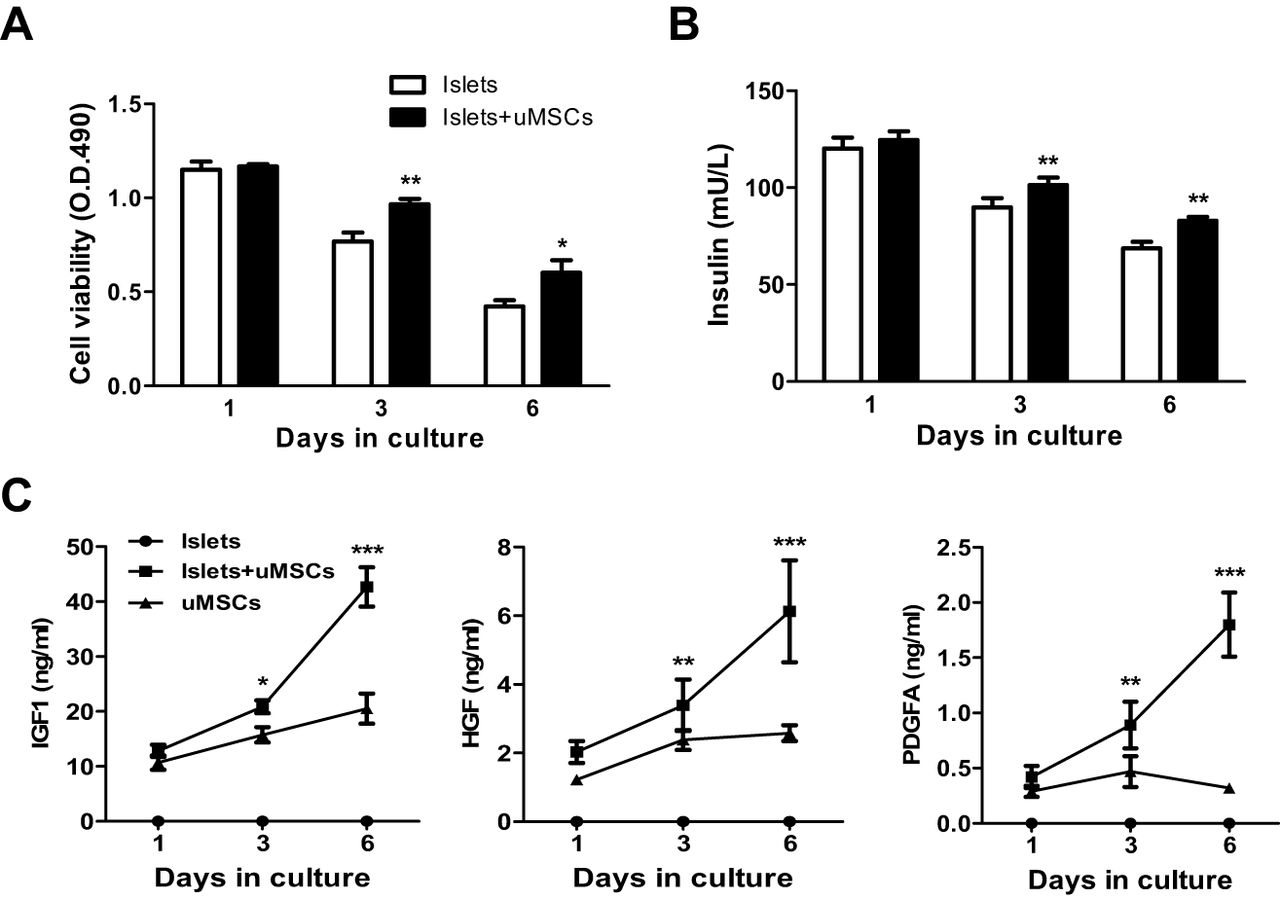
\includegraphics[width=7 cm]{fig2}
\caption{A: Apoptotic cell number per passage evaluated by TUNEL assay. B: hTERT expression determined by western blotting}
\label{Figure 2}
\end{figure}
\end{center}



\subsection{Average Cell Viability Levels (ACVL)}
Based on the results of the previously analyzed assays, ACVL was calculated for each cell passage. As shown in Figure 1E, the highest ACVL corresponded to P11, with high values also found at P14. As hDPSC were subcultured up to 20th subculture, the ACVL tended to gradually diminish until reaching its lowest value (lowest cell viability) at P19.

\subsection{Transferase dUTP nick end labeling (TUNEL) assay}
The number of apoptotic cells was determined by TUNEL assay in each hDPSC subculture (Figure 3A and 4). The percentage of apoptotic cells significantly increased from P15 to P17 (0.93 $\pm$ 0.38\% to 7.21 $\pm$ 2.07\%, p = 0.005) and continued increasing until the end of the study, when the top percentage of apoptotic cells was found (9.80 $\pm$ 6.08\%), showing a global trend to increase (p $<$ 0.001 for Friedman test) (Table 1).


\subsection{Western blot and inmunofluorescence}
Selected apoptosis and proliferation markers were analyzed by western blot and inmunofluorescence. Caspase 4 expression (pro-apoptotic marker) was slightly higher on P16 to P20 as compared to P11 to P15, especially at the end of the experiment (P18 to P20). Inmunofluorescence staining revealed a positive cytoplasmic pattern of expression, mainly at P19. BCL7C protein, related with anti-apoptotic activity, also presented a cytoplasmic pattern by inmunofluorescence and its expression was higher during the first five subcultures (P11 to P15), mainly at P14 and P15, determined by western blot and inmunofluorescence, and after that, expression decreased to almost absence.
PCNA is a well-known cell proliferation indicator. Its expression was higher at the beginning of the study (P11 to P15) and tended to slightly decrease as the hDPSC were subcultured (P16 to P20) (Figure 3B). Inmunofluorescence staining showed a typical nuclear pattern of expression mainly at P11, P13 and P15. Finally, telomerase activity determined by hTERT expression showed a slightly loss of expression at P17 and P19, as well as an increase at P15.

\newpage


\begin{landscape}
\begin{table}[htb]
\centering
\begin{tabular}{cccccccccccc}
\hline
\multicolumn{2}{c}{\textbf{CELL PASSAGE}}                                                                                               & \textbf{P11} & \textbf{P12} & \textbf{P13} & \textbf{P14} & \textbf{P15} & \textbf{P16} & \textbf{P17} & \textbf{P18} & \textbf{P19} & \textbf{P20} \\ \hline

\multicolumn{1}{c|}{\multirow{2}{*}{\textbf{\begin{tabular}[c]{@{}c@{}}TRYPAN BLUE\\  (\%)\end{tabular}}}}  & \multicolumn{1}{c|}{Mean} & 92.54        & 87.89        & 89.56        & 88.24                            & 85.61                            & 85.88                            & 89.97                            & 91.15                            & 75.94                            & 75.50                            \\

\multicolumn{1}{c|}{}                                                                                       & \multicolumn{1}{c|}{SD}   & 7.27         & 7.14         & 14.47        & 8.18                             & 6.62                             & 10.68                            & 7.68                             & 5.77                             & 23.09                            & 22.62                            \\ \cline{1-2}
\multicolumn{1}{c|}{\multirow{2}{*}{\textbf{\begin{tabular}[c]{@{}c@{}}WST-1\\ (Absorbance)\end{tabular}}}} & \multicolumn{1}{c|}{Mean} & 1.99         & 1.58         & 1.70         & 2.09                             & 1.93                             & 1.77                             & 1.83                             & 1.89                             & 1.79                             & 1.86                             \\
\multicolumn{1}{c|}{}                                                                                       & \multicolumn{1}{c|}{SD}   & 0.44         & 0.75         & 0.63         & 0.29                             & 0.51                             & 0.59                             & 0.64                             & 0.49                             & 0.71                             & 0.72                             \\ \cline{1-2}
\multicolumn{1}{c|}{\multirow{2}{*}{\textbf{\begin{tabular}[c]{@{}c@{}}LIVE/DEAD\\ (\%)\end{tabular}}}}     & \multicolumn{1}{c|}{Mean} & 90.20        & 92.67        & 91.81        & 92.70                            & 91.52                            & 89.81                            & 91.13                            & 89.68                            & 87.67                            & 89.57                            \\
\multicolumn{1}{c|}{}                                                                                       & \multicolumn{1}{c|}{SD}   & 7.63         & 5.63         & 3.33         & 3.41                             & 6.25                             & 4.74                             & 2.94                             & 9.64                             & 7.65                             & 5.69                             \\ \cline{1-2}
\multicolumn{1}{c|}{\multirow{2}{*}{\textbf{\begin{tabular}[c]{@{}c@{}}TUNEL\\ (\%)\end{tabular}}}}         & \multicolumn{1}{c|}{Mean} & 1.46         &              & 2.64         &                                  & 0.93                             &                                  & 7.21                             &                                  & 9.80                             &                                  \\
\multicolumn{1}{c|}{}                                                                                       & \multicolumn{1}{c|}{SD}   & 0.32         &              & 2.09         &                                  & 0.38                             &                                  & 2.07                             &                                  & 6.08                             &                                  \\ \hline
\end{tabular}
\caption{Analysis of cell viability at successive hDPSC passages (P1 to P10) according to trypan blue exclusion test, WST-1 assay and LIVE/DEAD assay.}
\label{Tabla 1}
\end{table}

\begin{table}[htb]
\centering
\begin{tabular}{cccccccccccc}
\hline
\multicolumn{2}{c}{\textbf{CELL PASSAGE}}                                                                                               & \textbf{P11} & \textbf{P12} & \textbf{P13} & \textbf{P14} & \textbf{P15} & \textbf{P16} & \textbf{P17} & \textbf{P18} & \textbf{P19} & \textbf{P20} \\ \hline

\multicolumn{1}{c|}{\multirow{2}{*}{\textbf{\begin{tabular}[c]{@{}c@{}}TRYPAN BLUE\\  (\%)\end{tabular}}}}  & \multicolumn{1}{c|}{Mean} & 92.54        & 87.89        & 89.56        & 88.24                            & 85.61                            & 85.88                            & 89.97                            & 91.15                            & 75.94                            & 75.50                            \\

\multicolumn{1}{c|}{}                                                                                       & \multicolumn{1}{c|}{SD}   & 7.27         & 7.14         & 14.47        & 8.18                             & 6.62                             & 10.68                            & 7.68                             & 5.77                             & 23.09                            & 22.62                            \\ \cline{1-2}
\multicolumn{1}{c|}{\multirow{2}{*}{\textbf{\begin{tabular}[c]{@{}c@{}}WST-1\\ (Absorbance)\end{tabular}}}} & \multicolumn{1}{c|}{Mean} & 1.99         & 1.58         & 1.70         & 2.09                             & 1.93                             & 1.77                             & 1.83                             & 1.89                             & 1.79                             & 1.86                             \\
\multicolumn{1}{c|}{}                                                                                       & \multicolumn{1}{c|}{SD}   & 0.44         & 0.75         & 0.63         & 0.29                             & 0.51                             & 0.59                             & 0.64                             & 0.49                             & 0.71                             & 0.72                             \\ \cline{1-2}
\multicolumn{1}{c|}{\multirow{2}{*}{\textbf{\begin{tabular}[c]{@{}c@{}}LIVE/DEAD\\ (\%)\end{tabular}}}}     & \multicolumn{1}{c|}{Mean} & 90.20        & 92.67        & 91.81        & 92.70                            & 91.52                            & 89.81                            & 91.13                            & 89.68                            & 87.67                            & 89.57                            \\
\multicolumn{1}{c|}{}                                                                                       & \multicolumn{1}{c|}{SD}   & 7.63         & 5.63         & 3.33         & 3.41                             & 6.25                             & 4.74                             & 2.94                             & 9.64                             & 7.65                             & 5.69                             \\ \cline{1-2}
\multicolumn{1}{c|}{\multirow{2}{*}{\textbf{\begin{tabular}[c]{@{}c@{}}TUNEL\\ (\%)\end{tabular}}}}         & \multicolumn{1}{c|}{Mean} & 1.46         &              & 2.64         &                                  & 0.93                             &                                  & 7.21                             &                                  & 9.80                             &                                  \\
\multicolumn{1}{c|}{}                                                                                       & \multicolumn{1}{c|}{SD}   & 0.32         &              & 2.09         &                                  & 0.38                             &                                  & 2.07                             &                                  & 6.08                             &                                  \\ \hline
\end{tabular}
\caption{Analysis of cell viability at successive hDPSC passages (P1 to P10) according to trypan blue exclusion test, WST-1 assay and LIVE/DEAD assay.}
\label{Tabla 2}
\end{table}
\end{landscape}

\section{Discussion}
Lorem \cite{RN45} ipsum aemet\cite{RN394} dolor aenean molestie, nisi sit amet lobortis posuere, felis lacus malesuada ante, vel luctus nisl orci eleifend ligula. Pellentesque est magna, placerat a diam ultricies, pretium tincidunt orci. Nullam turpis enim, dictum sit amet molestie non, volutpat ut sapien. Mauris nisl diam, varius et maximus non, varius nec dui. Sed quis tempor enim, non luctus dolor. Donec laoreet feugiat odio ac facilisis. Quisque ut tellus et nulla mattis tristique eu a nulla. Cras sollicitudin lorem vel ipsum viverra, eget convallis tortor pellentesque. Nullam consectetur nisl tincidunt nisi vestibulum feugiat \cite{RN420,RN877}. Praesent ac egestas turpis. Cras quis hendrerit magna. Morbi sed lorem id eros elementum condimentum.\\
Duis non nisi mollis, dignissim metus sit amet, ultricies enim. Praesent et ligula urna. Integer tristique magna at aliquet posuere. Ut consectetur, sem id sollicitudin accumsan, libero quam congue nisl, vel tempus orci dolor quis felis. Maecenas nisl tortor, gravida ut luctus ut, luctus et leo. Aliquam erat volutpat. Donec dapibus lorem turpis, et imperdiet erat egestas eget. Fusce non tellus augue. Phasellus facilisis tincidunt felis in vulputate. Vestibulum dignissim luctus ullamcorper. Etiam viverra odio id arcu egestas, id pellentesque quam vulputate \cite{RN1039,RN795,RN962}. Vivamus et leo eleifend, porta magna et, suscipit felis. Aenean sapien felis, mollis a nunc quis, mattis tempor erat. Aenean tristique erat libero, in vestibulum urna efficitur ac. Proin interdum viverra elit sed fringilla.\\
Curabitur semper luctus quam. Aenean vitae tellus et sem bibendum tincidunt at in nisi. In eget mi vel leo lacinia ornare in ac tellus. Sed vitae mi tempus, ullamcorper purus ac, porttitor tellus. Sed at rutrum mi. Aliquam quis rhoncus urna. Fusce lobortis mi tempus, porta enim sit amet, eleifend massa. In vitae eros tortor. Lorem ipsum dolor sit amet, consectetur adipiscing elit. Vestibulum semper lobortis eros, sed vestibulum mauris scelerisque et. Vivamus suscipit interdum lorem, sed fringilla odio gravida a. Mauris ultrices sem metus, quis sodales erat lacinia ac \cite{RN632}. Maecenas imperdiet sollicitudin neque a interdum. Aenean dui velit, molestie quis ante eget, finibus egestas ex. Sed eros nunc, tristique in purus sit amet, tempus pellentesque purus. Aliquam libero odio, feugiat vitae commodo et, varius nec dolor.\\
Nullam ullamcorper justo eu ullamcorper euismod. Nulla interdum augue laoreet, suscipit nunc non, gravida purus. Quisque sollicitudin mi eu justo consequat semper. Nullam malesuada vehicula dolor, luctus ornare mauris malesuada nec. Cras a tempus nisl \cite{RN398}. Curabitur et turpis diam. Nam porta lacinia nibh vitae tincidunt. Ut leo quam, aliquam sit amet mauris eget, convallis dictum odio \cite{RN1022}. Sed quis euismod nunc. Interdum et malesuada fames ac ante ipsum primis in faucibus. Nullam egestas tristique augue non suscipit. Vestibulum ante ipsum primis in faucibus orci luctus et ultrices posuere cubilia Curae; Praesent bibendum rhoncus neque, sit amet elementum odio. Sed porta dui eu quam lobortis, ac bibendum ligula rutrum. Ut vel tellus quam \cite{RN635,RN1142}.\\
Mauris non tristique eros. Ut ut lorem molestie felis placerat lobortis id vel nulla. Morbi auctor neque imperdiet sapien sollicitudin, id scelerisque velit feugiat. Suspendisse potenti. Donec sit amet tortor aliquam, volutpat ligula et, sagittis augue. Cras et molestie nibh. In mollis augue nisl, accumsan maximus nisi ultrices eu. Orci varius natoque penatibus et magnis dis parturient montes, nascetur ridiculus mus. Nam iaculis sapien pharetra, eleifend orci faucibus, porttitor erat. Praesent varius leo velit, in iaculis orci tincidunt at. In sit amet tellus vestibulum sem tincidunt convallis sodales eu mi. Nam et posuere neque. In hac habitasse platea dictumst. Nam metus magna, lobortis a consectetur a, sollicitudin eu ipsum. Vestibulum a sodales tortor. Donec ornare, nulla at aliquet vehicula, sem metus pharetra lectus, at sollicitudin arcu elit et ligula.\\

\section{Acknowledgements}
This study was supported by the Spanish Plan Nacional de Investigación Científica, Desarrollo e Innovación Tecnológica (I+D+I) from the National Ministry of Science and Innovation (Instituto de Salud Carlos III), grants FIS PI11/1582 and PI11/2668.

%\addcontentsline{toc}{section}{References}
\bibliographystyle{acm}
\bibliography{bibliografia}

\end{document}